\subsection{Overview}
This section is dedicated to the implementation, integration and test plan. The first part of this section will be dedicated to the identification of the main features of the system and the definition of the components that will be used to implement them. The second part will be dedicated to the integration and testing of the components. The third part will be dedicated to the system testing. The last part will be dedicated to the additional specifications on testing.
\subsubsection{Features identification}
The following list describes the main features of the system and the components that will be used to implement them:
\begin{itemize}
    \item \textbf{User registration and login}: this feature will be implemented by the WebApp and by two componenets that belongs to the Application Server: the RegistrationManager and the LoginManager. The WebApp will provide the user interface for the registration and login process. The RegistrationManager will provide the logic for the registration while the LoginManager will take care of the login process.
    \item \textbf{Creation of a Tournament}: this feature is an educator only feature. It will be implemented by the WebApp to insert the details and restrictions about the tournament, by the AuthorizationManager in order to check if the user is an educator and finally by the TournamentManager. The WebApp will provide the user interface for the creation of a tournament. The TournamentManager will provide the logic for the creation of a tournament.
    \item \textbf{Creation of a Battle}: this feature is an educator only feature. It will be implemented by the WebApp to insert the details and restrictions about the battle, by the AuthorizationManager in order to check if the user is an educator, by the BattleManager and its subcomponent: the CodeKataManager. Finally, since every battle must have their own GitHub repository the BattleManager will also handle the communication with the external system GitHub in order to create the repository for the battle. The WebApp will provide the user interface for the creation of a battle. The CodeKataManager will take care of the creation of the Code Kata while the BattleManager will provide the logic for the creation of a battle.
    \item \textbf{Manage Team}: this feature is a student only feature. It will be implemented by the WebApp to provide the name of the team and also to select the student to invite to the team. The AuthorizationManager will check if the user is a student, the TeamManager will provide the logic for the creation of a team. The BattleManager will be used to associate the newly created team with the battle of interest. The WebApp will provide the user interface for the creation of a team. Additionally the invitiation to join a team is handled by the InvitationManager.
    \item \textbf{Automatic Evaluation}: this feature is one of the most important features of the system. The implementation of this feature will be achieved by the use of the SubmissionManager, EvaluationManager and GitHub. The SubmissionManager will take care of the submission done by the Team on the forked GitHub repository of the battle. The EvaluationManager is responsible for the running of the automatic evaluation on the submitted code. The automatic evaluation starts when the GitHub action set up by the Team is triggered by a push on the forked repository. When the GitHub action is triggered it will call an API endpoint that will start the evaluation process. Finally, there is the RankingMaanger that will take care of the ranking of the students for the battle.
    \item \textbf{Manual Evaluation}: this feature is an educator only feature. It will be implemented by the WebApp to provide the educator with the possibility to manually update the score of an evaluation. The AuthorizationManager will check if the user is an educator. The EvaluationManager is the component that will be used to update the score of an evaluation. Finally, there is the RankingMaanger that will take care of the update of the ranking of the students for the battle.
    \item \textbf{Educator Invitation}: this feature is an educator only feature. It will be implemented by the WebApp to provide the educator with the possibility to invite other educators to join a tournament. The AuthorizationManager will check if the user is an educator. The InvitationManager will take care of the invitation process. Finally the TorunamentManager will be used to associate the invited educator with the tournament if the invitation is accepted.
    \item \textbf{Notification of the user}: the notification feature is trasversal to multiple features. These features are: the creation of a tournament, the creation of a battle, the invitation to join a team, the invitation to join a tournament. The NotificationManager will be used to send the notification to the user. The WebApp will provide the user interface to view the notifications.
\end{itemize}
\subsubsection{Implementation, Integration and Test Plan}
The system is composed by the following subsystems:
\begin{itemize}
    \item \textbf{WebApp}
    \item \textbf{WebServer}
    \item \textbf{Application Server}
    \item \textbf{DBMS}
    \item \textbf{External Services}: GitHub
\end{itemize}
These subsystems are developed, tested, and integrated using a bottom-up approach.
The bottom-up strategy begins at the granular level, focusing on the creation and development of individual components or modules. Each of these elements is designed and developed in isolation, allowing for a deep focus on functionality and performance. This approach ensures that every component is robust and fully operational before it becomes part of a larger system. 

Once these individual modules are developed, they undergo rigorous testing to identify and rectify any issues early in the development cycle. This early detection of problems is a key advantage, as it significantly reduces the complexity and cost of fixes later on. 

After ensuring the reliability of each component, the process moves to the integration phase. Here, these independently developed modules are gradually assembled to form larger subsystems. This step-by-step assembly allows for careful monitoring of interactions between components, ensuring overall system coherence and performance.

Finally, these subsystems are integrated to complete the overall system or project. This incremental approach not only facilitates detailed scrutiny at each stage but also allows for parallel development of components, accelerating the overall timeline. Additionally, it provides flexibility in adapting to changes or incorporating new technologies as development progresses. 

This method emphasizes the significance of various functionalities while aiming to deliver a tangible application feature at each stage of the plan. For each subsystem, we will focus on the implementation, integration, and testing of its constituent components.

It's important to note that components belonging to external systems are not subject to implementation and testing within our plan. These external components are assumed to be reliable and are treated as such.

The following diagrams shows the order in which the components will be implemented, integrated and tested. The arrows represent the dependencies between the components. The components that are not connected by an arrow are independent and can be implemented, integrated and tested in any order.

\subsubsection*{Submission and Evaluation service}
The main components of the Submission and Evaluation service are the SubmissionManager, EvaluationManager, RankingManager and the DBMS Component. The SubmissionManager depends on the EvaluationManager, the RankingManager depends on the EvaluationManager and the DBMS and the the RankingManager depends on the DBMS.
\begin{figure}[H]
    \centering
    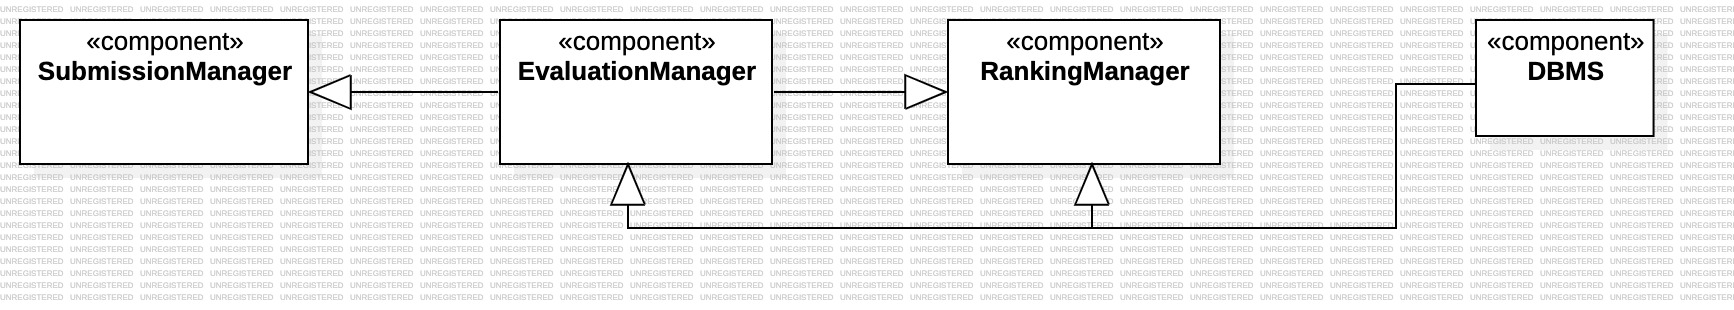
\includegraphics[width=\textwidth]{Diagrams/SubmissionIntegrationPlan.jpg}
    \caption{Submission and Evaluation service}
    \label{fig:submission_and_evaluation}
\end{figure}

\subsubsection*{Notification service}
The main components of the Notification service are the DBMS, the NotificationManager, the TournamentManager, the BattleManager and the InvitationManager. The NotificationManager depends on the DBMS. The TournamentManager, BattleManager and InvitationManager depend on the NotificationManager.
\begin{figure}[H]
    \centering
    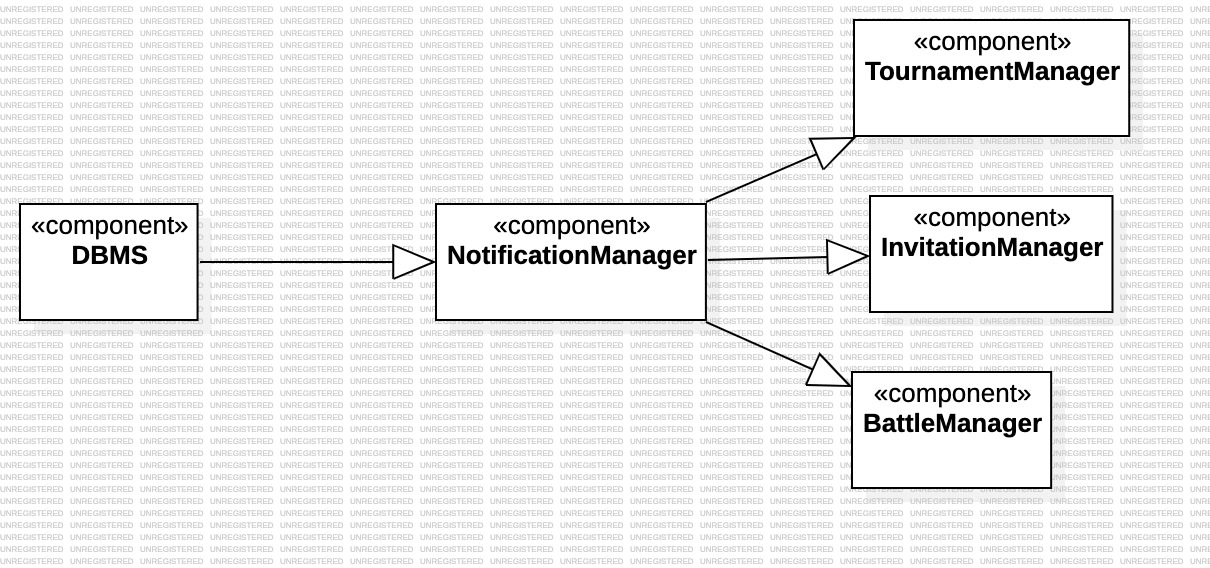
\includegraphics[width=\textwidth]{Diagrams/NotificationIntegrationPlan.jpg}
    \caption{Notification service}
    \label{fig:notification}
\end{figure}
\clearpage
\subsubsection*{Authorization service}
Regarding the Authorization service, the main component is the AuthorizationManager that depends on the TeamManager, the TournamentManager, the BattleManager, the InvitationManager and the EvaluationManager.
\begin{figure}[H]
    \centering
    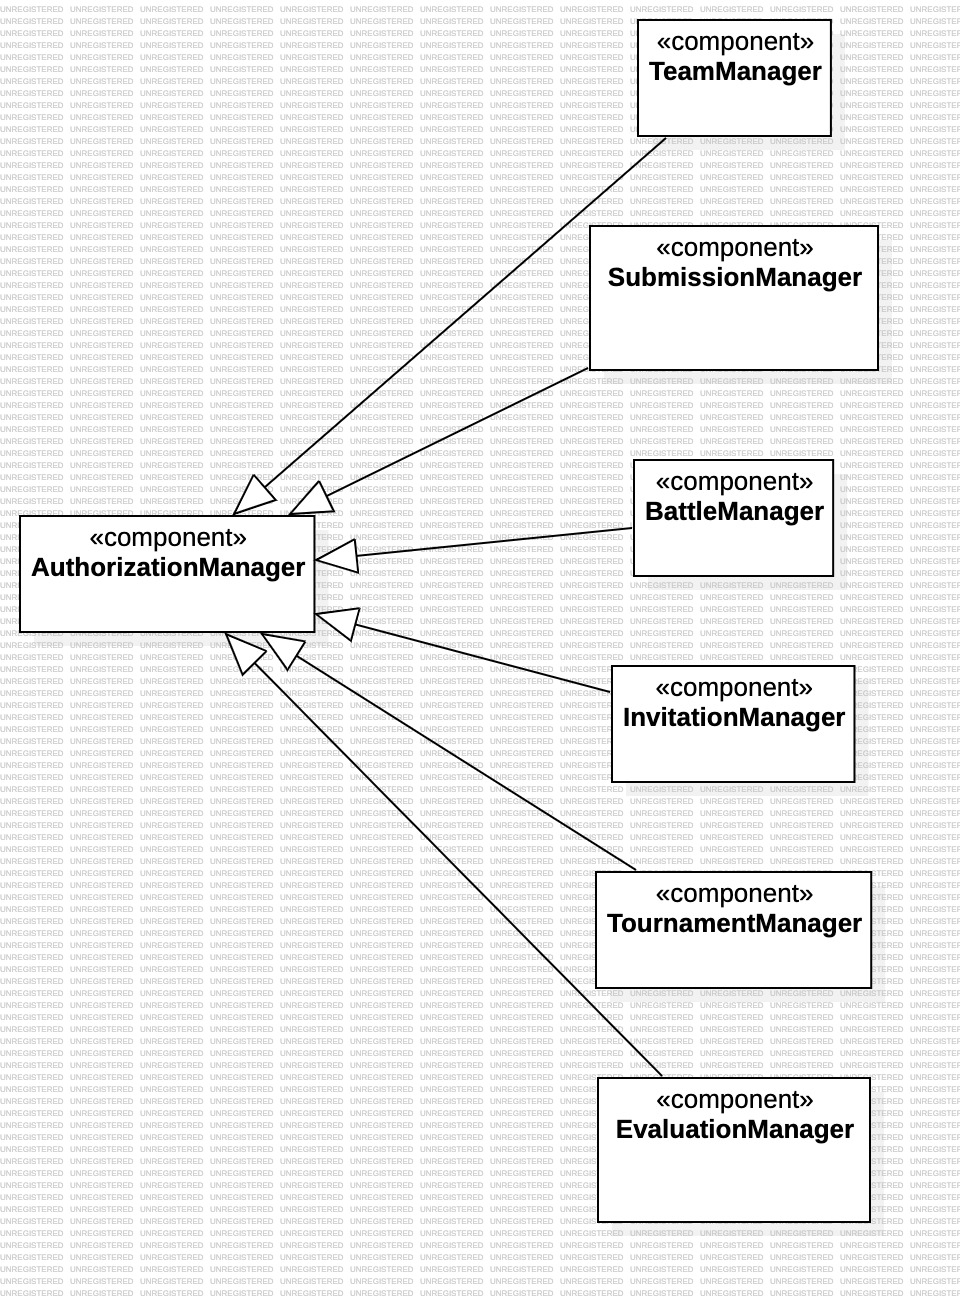
\includegraphics[width=0.6\textwidth]{Diagrams/AuthorizationIntegrationPlan.jpg}
    \caption{Authorization service}
    \label{fig:authorization}
\end{figure}
\clearpage
\subsubsection*{Dispatcher service}
The Dispatcher service is composed by the APIGateway, in order to dispatch the requests to the correct component it needs the AuthorizationManager, LoginManager, RegistrationManager and the RankingManager.
Since the APIGateway dispatches the requests to the correct component, its development and integration can be done using a thread approach. With this approach the functionalities of the APIGateway can be implemented and tested in parallel with the development of the other components.
\begin{figure}[H]
    \centering
    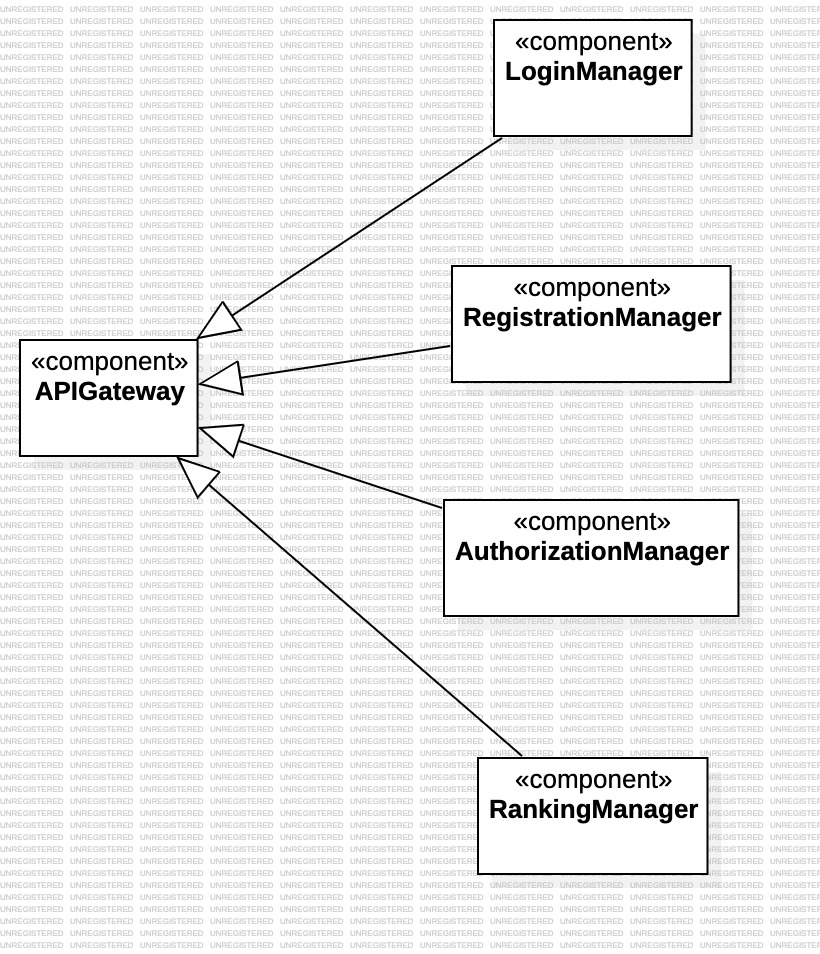
\includegraphics[width=0.6\textwidth]{Diagrams/DispatcherIntegrationPlan.jpg}
    \caption{Dispatcher service}
    \label{fig:dispatcher}
\end{figure}
\clearpage
\subsubsection*{System integration}
The system integration is the last step of the implementation and the integration. The system integration is composed by the integration of the WebApp, WebServer, Application Server and the DBMS. The WebApp depends on the WebServer, the WebServer depends on the Application Server and the Application Server depends on the DBMS. Finally for the external services we have GitHub that depends on the Application Server.
\begin{figure}[H]
    \centering
    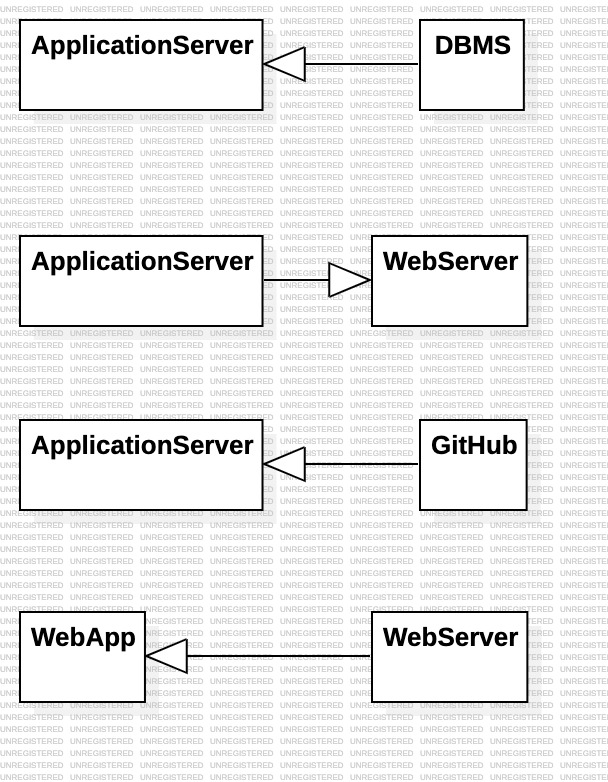
\includegraphics[width=0.5\textwidth]{Diagrams/SystemIntegrationPlan.jpg}
    \caption{System integration}
    \label{fig:system_integration}
\end{figure}
\clearpage
\subsection{System testing}

The primary objective of system testing is to validate the complete and integrated software system to ensure that it meets the specified requirements. This phase is critical to ensure that the system operates as intended in its real-world environment.\\
The system testing phase will be conducted in accordance with the following plan:
\begin{itemize}
    \item \textbf{Functional Testing:} To check if the system performs all the functions specified in the RASD document correctly.
    \item \textbf{Performance Testing:} To assess the system’s stability and responsiveness under various conditions. A useful benchmark for the CKB Platform is to evaluate the time taken to process a submission, build the project, run the tests and return the results. By analyzing the results of this tests we can discover bottlenecks and optimize the system accordingly.
    \item \textbf{Security Testing:} To ensure the system's features designated for a specific role are accessible only to users with that role, as well as to identify and address any commond vulnerabilities specified in the ``OWASP Top Ten''.
    \item \textbf{Load Testing}: To evaluate the system's performance under extreme workloads. Useful test cases for the CKB Platform is to simulate a large number of concurrent submissions and consequently evaluations.
    \item \textbf{User Acceptance Testing (UAT):} To confirm that the system meets the end-user requirements and is ready for deployment.
\end{itemize}

\subsubsection{Test Environment}
The testing environment is not particularly demanding since for the client side we only need a browser that support HTML, CSS and Javascript and for the server side it is necessary a basic server that supports the execution of an hypervisor for the virtualization in order to virtualize the EvaluationManager component. There are no strict requirements on the hardware because it depends on the number of users that will use the system and it will be calibrated according to the load test phase also.
\subsection{Review and Approval}
The testing phase will conclude with a review process, involving the development team, project manager, and key stakeholders. The system will be approved for deployment upon successful completion of all test scenarios and resolution of any critical issues.